% !TEX program = lualatex
\documentclass[11pt]{article}

% -------- LuaLaTeX : polices et langue --------
\usepackage{fontspec}
\setmainfont{Latin Modern Roman}
\setsansfont{Tex Gyre Heros}
%\renewcommand{\familydefault}{\sfdefault} % force le sans serif par défaut
\usepackage{polyglossia}
\setdefaultlanguage{french}

% -------- Mise en page --------
\usepackage[a5paper, margin=1cm]{geometry}
\usepackage{multicol}
\usepackage{fancyhdr}
\pagestyle{empty}
\usepackage[most]{tcolorbox}

% -------- Mathématiques --------
\usepackage{amsmath,amssymb,mathtools}
% \usepackage{siunitx}
% \sisetup{locale=FR}

% Charger une police emoji
\newfontface\emoji{NotoColorEmoji}[Renderer=Harfbuzz]

\newcommand{\ligne}{{\color{gray!60}\hrulefill}}

\usepackage{enumitem}
\usepackage{ProfCollege}

% -------- Divers --------
\setlength{\parindent}{0pt}
\setlength{\parskip}{.8em}
\begin{document}

\begin{tcolorbox}[colback=teal!10!white, colframe=teal!80!black]
\begin{center}
\large\textbf{Jeu de Juniper Green {\emoji 🧗}}
\end{center}
\end{tcolorbox}

\vspace{1.5em}

On peut représenter le jeu de Juniper Green (version 1 joueur) par un \emph{graphe} dans lequel deux \emph{sommets} sont reliés par une \emph{arête} si et seulement si l’un des deux divise l’autre.

On ne tracera pas les arêtes reliées au sommet $1$ pour ne pas surcharger le graphe, mais puisque $1$ divise tous les nombres entiers il est bien sûr relié à tous les autres sommets. 

Trouver une partie la plus longue possible revient alors à trouver un \emph{chemin} le plus long possible le long des arêtes du graphe sans passer deux fois par le même sommet (sans oublier que $1$ est connecté à tous les autres sommets).

\section*{Nombres entiers de 1 à 16}

\begin{center}
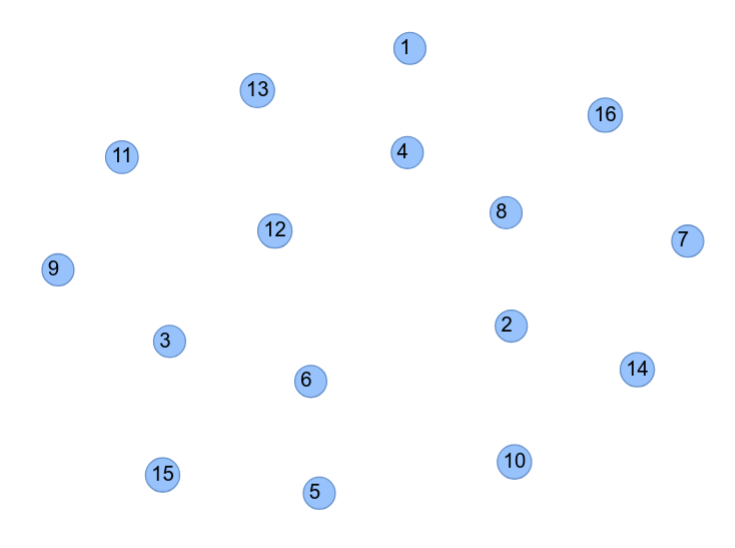
\includegraphics[width=12cm]{Images/Juniper16False.png}
\end{center}

Un chemin le plus long : \ligne

\newpage

\section*{Nombres entiers de 1 à 20}

\begin{center}
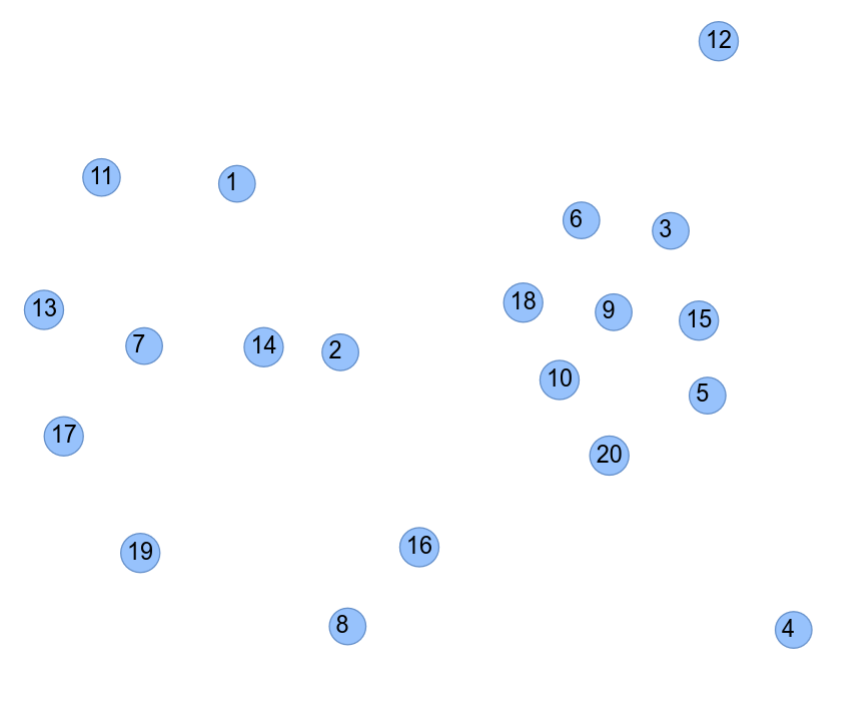
\includegraphics[width=12cm]{Images/Juniper20False.png}
\end{center}

\ligne

\newpage

\section*{Nombres entiers de 1 à 25}

\begin{center}
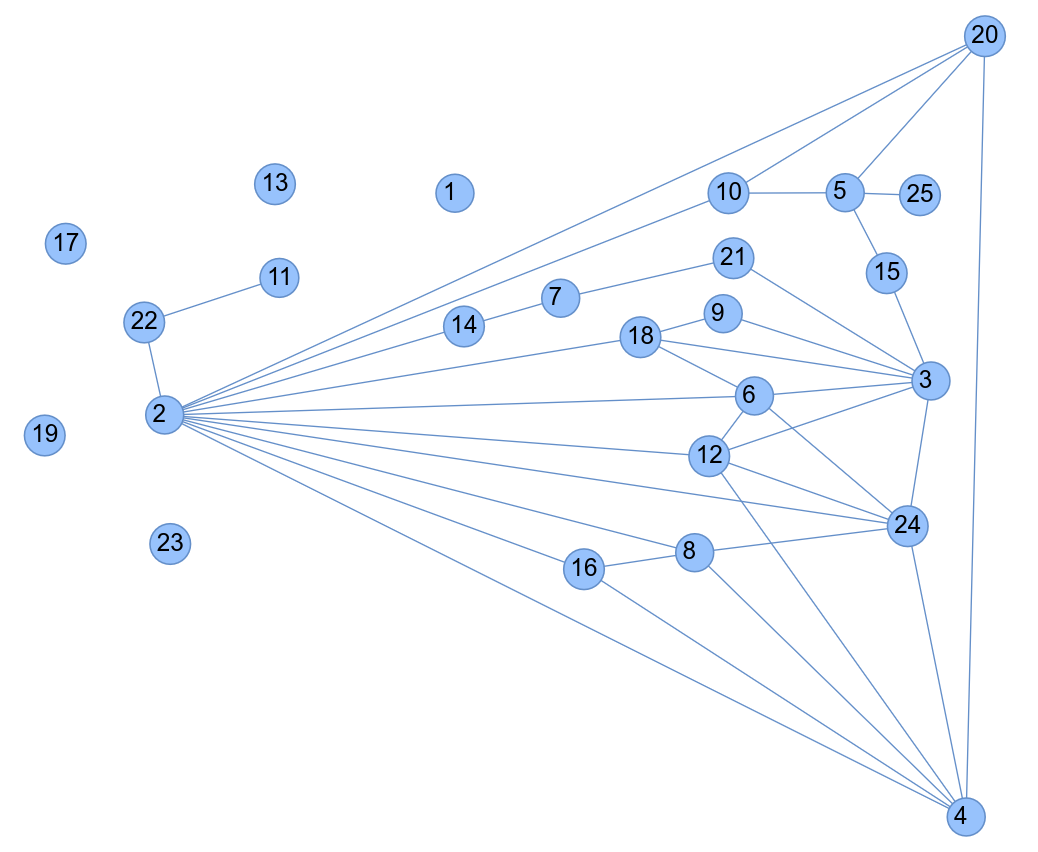
\includegraphics[width=\linewidth]{Images/Juniper25True.png}
\end{center}

\ligne

\end{document}
